\newpage
\subsubsection{ESP}
\label{subsubsec:ESP}

Für die Implementierung des kabellosen Zugriffs wird das ESP32 verwendet. Die Hauptfunktion auf dem Print ist die Kommunikation mit dem Mikrocontroller über die zweite serielle Schnittstelle. Die Ansteuerung zum Schreiben des Programmspeichers wird so implementiert, dass der Boot-Modus automatisch gestartet werden kann, wenn ein Code hochgeladen werden soll. Dies hat eine zusätzliche Schaltung zur Folge.

Aufgrund schon bestehender Erfahrungen wurde ein Espressif ESP-Modul ausgewählt. Grundsätzlich standen zwei Modelle zur Auswahl. Das ESP8266 und das ESP32. Für die Cocktailmaschine wurde das ESP32 ausgewählt, da diese leistungsstärker ist. Die genauen Datenvergleiche sind im Anhang Kapitel \ref{Appendix:ESP32_vs_ESP8266} ersichtlich. Das ESP32 unterstützt das Protokoll nach ISO 802.11 b/g/n und kann somit auf 2.4GHz sowie 5GHz arbeiten. Mit dem n-Protokoll und einer Antenne kann so bis zu 150MBit übertragen werden bei einer Bandbreite von 20MHz.

Wichtig ist, dass ein ESP ausgewählt wird, welches einen Anschluss für eine abgesetzte Antenne hat, da die Leiterplatte, worauf das Modul verbaut wird, im Gehäuse platziert wird. Dazu eignet sich der Espressif ESP32-32U.

Im Anhang Kapitel \ref{Appendix:ESP32_Strapping} sind die Strapping-Pins aufgelistet, welche während dem Startvorgang einen Einfluss auf die Konfiguration des ESP32 haben. Mit diesen Pins kann die Ausgangsspannung des internen Spannungsregler für VDD\_SDIO, der Bootmodus, der Debug-Log-Print während dem Booten sowie das SPI-Timing der Kommunikation mit der SDIO-Schnittstelle des ESP32 konfiguriert werden. Eine genauere Beschreibung der Pins befindet sich im selben Kapitel.

%\begin{figure}[!h]
%\center
%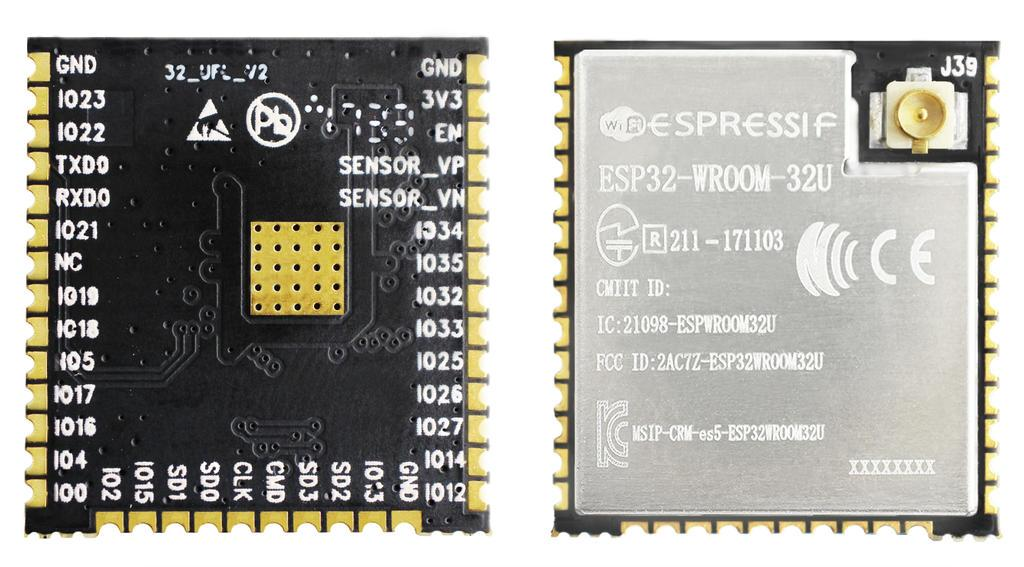
\includegraphics[width = 0.4\textwidth]{graphics/Produktbild_ESP32}
%\caption{ESP32-32U Wroom.}
%\label{fig:Produktbild_ESP32_32U_Wroom}
%\end{figure}
%
%\begin{figure}[!h]
%\center
%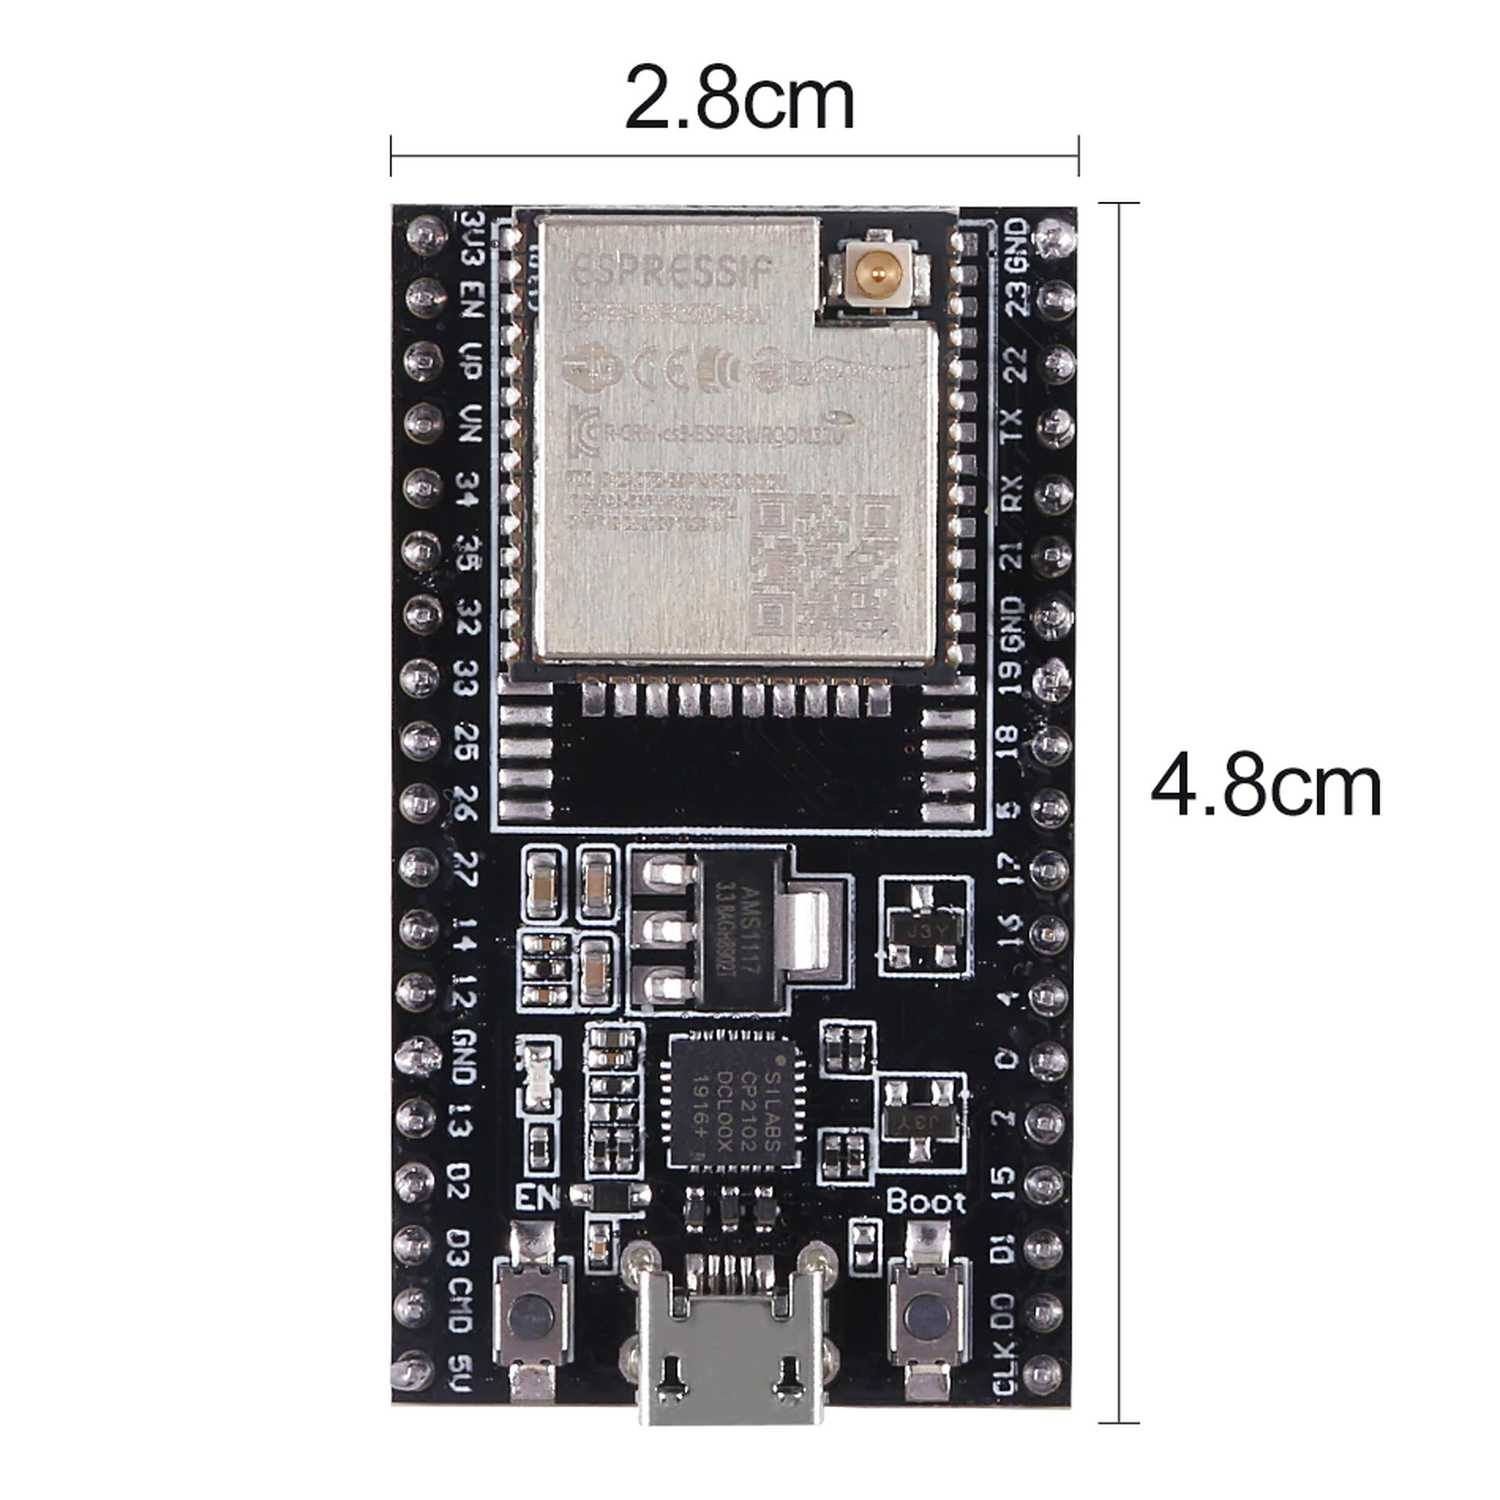
\includegraphics[width = 0.4\textwidth]{graphics/Produktbild_ESP32_2}
%\caption{ESP32-32U DevKit.}
%\label{fig:Produktbild_ESP32_32U_DevKit}
%\end{figure}

\paragraph{Schema (Bluetooth- / Wifimodul)}\mbox{}

In Abbildung \ref{fig:Schema_ESP32} wird das Schema rund um das ESP32 an sich gezeigt. Es beinhaltet Stützkondensatoren sowie einige Pull-up- und Pull-down-Widerstände, welche verwendet werden, um einen vordefinierten Grundzustand beim Booten des ESP32-Moduls zu erreichen (Strapping-Pins). Weiter gibt es einen Kondensator, welcher dazu da ist, bei gewünschter Zeit in den Download-Boot-Modus zu gelangen. In diesem Modus kann die User-Applikation übertragen werden.

\begin{figure}[H]
	\centering
	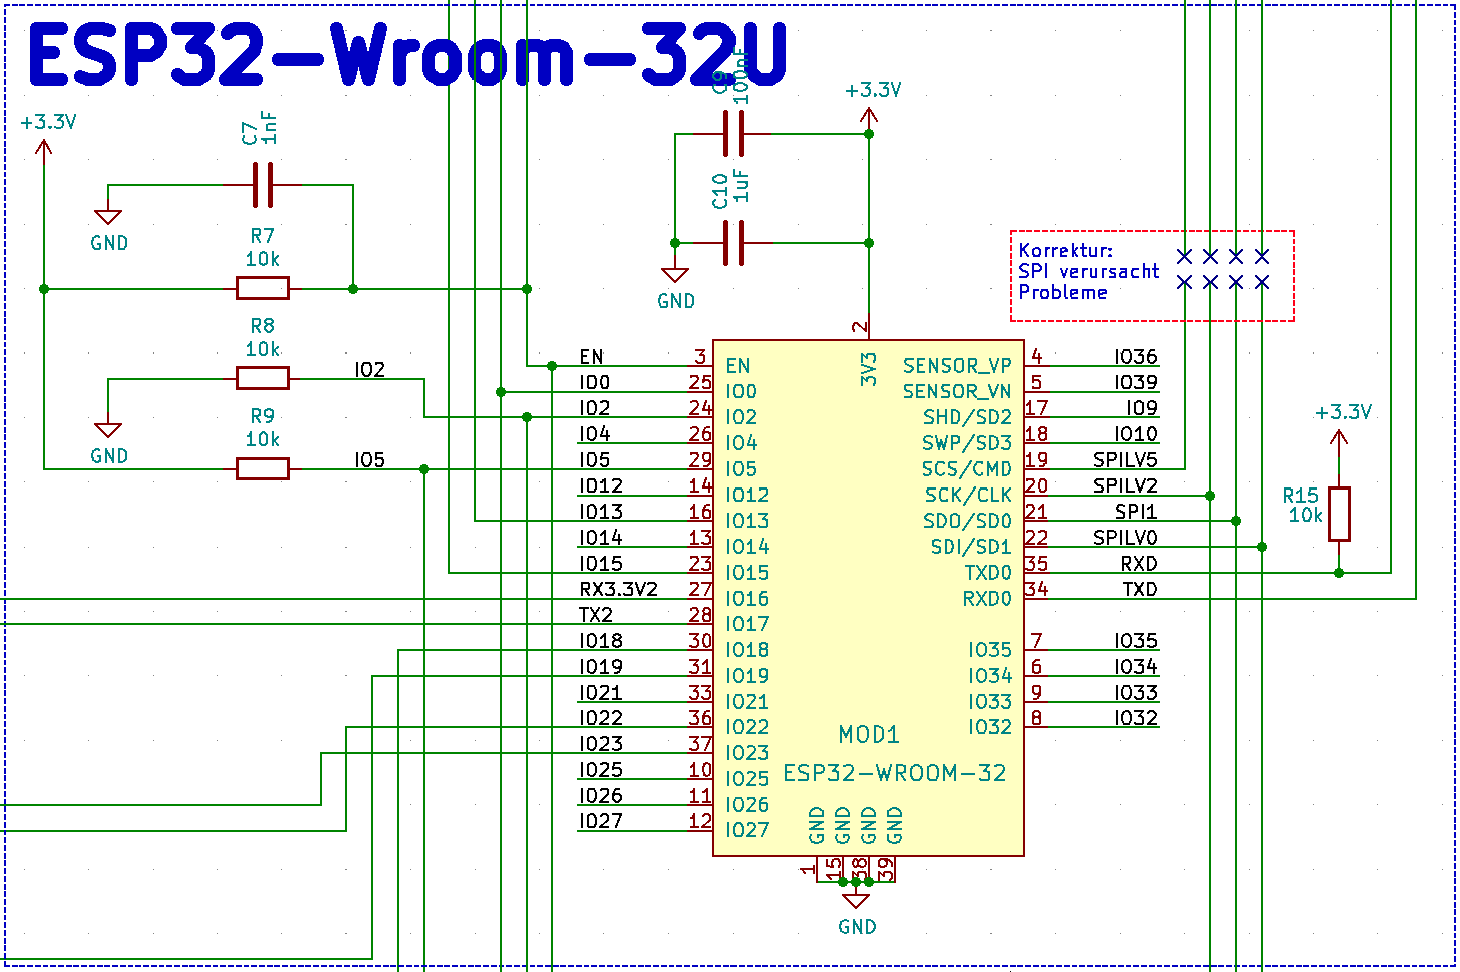
\includegraphics[width=0.8\textwidth]{graphics/Schema_ESP32}
	\caption{Schema ESP32-Wroom-32U.}
	\label{fig:Schema_ESP32}
\end{figure}

\paragraph{Funktionsbeschrieb der Schaltung (Bluetooth- / Wifimodul)}\mbox{}

Das ESP32 an sich ist mit MOD1 beschriftet. Die Kondensatoren C9 und C10 dienen zur Glättung der Eingangsspannung. Über den EN-Pin wird das Modul ein- und ausgeschaltet (acitve high), der Widerstand R7 zieht diese Leitung auf 5V. Die Widerstände R8, R9, R10 und R11 sind an die Strapping-Pins angeschlossen.
%Über diese werden beim Aufstarten des ESP32 der Boot-Modus, die Versorgungsspannung von VDD\_SDIO\footnote{Secure Digital Input Output}-Slave (Erweiterung der SD-Spezifikationen) und andere Initialisierungseinstellungen konfiguriert.
Details zu den Konfigurationen sind in Tabelle \ref{tab:Strapping_pins} aufgelistet\footnote{https://www.espressif.com/sites/default/files/documentation/esp32\_datasheet\_en.pdf S.13}. Der Widerstand R15 zieht U0TXD auf HIGH. Aus Tabelle \ref{tab:Einfluss_Pins_auf_Boot_Modus} ist ersichtlich, dass dieser für den normalen Boot-Modus auf HIGH sein muss. Für den Download-Boot-Modus hat dieser kein Einfluss. Mit dem Kondensator C7 wird sichergestellt, dass nach einem Reset der Download-Boot-Modus gestartet werden kann. Die Interaktion zwischen Computer und ESP32 wird auch Handshake genannt. Wie dieser genau funktioniert, wird in Kapitel \ref{subsubsec:Handshake_ESP32} erklärt.

%Wird der Reset-Pin au LOW gezogen, so entlädt sich der Kondensator. Sobald der Reset-Pin auf HIGH gezogen wird, dauert es länger, bis ein logic High-Zustand am CMOS-Eingang erkannt wird. Wird der Pin IO0 auf LOW gezogen, bevor der Enable-Pin nach einem Reset einen HIGH-Zustand erreicht, so wird das ESP32 in den Download-Boot-Modus gesetzt. Das Setzen

\paragraph{Schema (Automatische Boot-Logik)}\mbox{}

In Abbildung \ref{fig:Schema_ESP32_Flashbuttons} wird die Schaltung gezeigt, welche verwendet wird, das ESP32-Modul in den gewünschten Boot-Zustand zu bringen. Für die Beschaltung der automatischen Boot-Logik benötigt es eine Schaltung mit DTR und RTS als Inputs vom USB-UART-Converter her und EN und IO0 als Outputs auf das ESP32. Die Buttons können bei Bedarf verwendet werden, sind für den automatischen Boot-Modus jedoch nicht zwingend nötig. Sie könnten dazu verwendet werden manuell in den Bootmodus zu gelangen.\\
Die Widerstände R20 und R21 sind Vorwiderstände an der Basis der Transistoren Q1 und Q2. R22 und R23 sind Pull-Up-Widerstände für die EN- und IO0-Leitung. Die Kondensatoren C13 und C12 dienen zum entprellen. Die Widerstände R25 und R24 begrenzen den Strom bei Drücken der Buttons S1 und S2.

\todo{Quelle nicht in Fusszeile sondern richtig ins Quellenverzeichnis}

\begin{figure}[H]
	\centering
	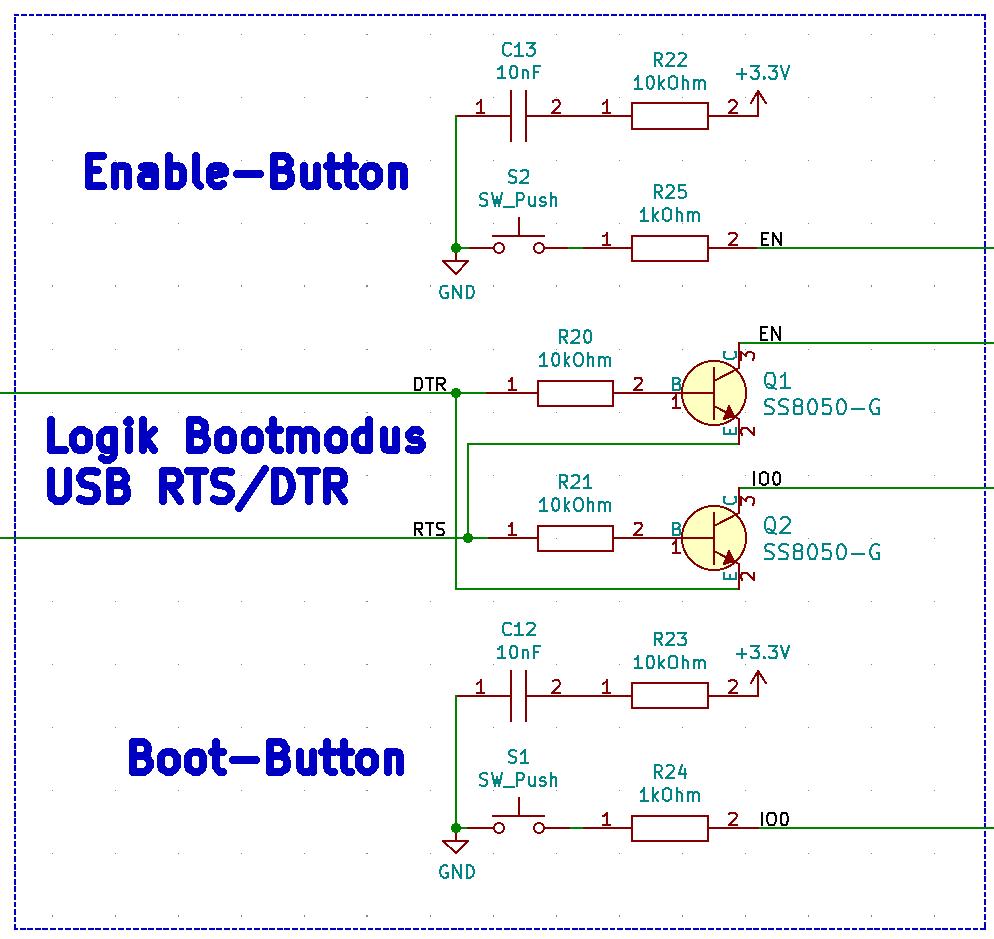
\includegraphics[width=0.7\textwidth]{graphics/Schema_ESP32_Flashbuttons}
	\caption{Schema ESP32-Wroom-32U.}
	\label{fig:Schema_ESP32_Flashbuttons}
\end{figure}

\paragraph{Funtionsbeschrieb der Schaltung (Automatische Bootlogik)}\mbox{}

Mit der automatischen Bootlogik werden die Pins EN und IO0 so angesteuert, sodass das ESP32 automatisch neu gestartet wird und der Download-Boot-Modus gestartet wird. Das Verhalten des ''Auto Program Cirquit'' und eine detailierte Beschreibung des Vorgangs ist im Anhang Kapitel \ref{Appendix:Handshake_ESP_Messung} zu finden. Darin wird erklärt, auf welche Weise die DTR- und RTS-Leitung geschaltet werden müssen, damit die EN- und IO0-Leitung richtig gesetzt werden.